%
% teil6.tex -- Anwendung, die Kepler-Gleichung
%
% (c) 2026 Gian Cavegn, OST Ostschweizer Fachhochschule
%
% !TEX root = ../../buch.tex
% !TEX encoding = UTF-8
% !TeX spellcheck = de_CH
%
\section{Die Kepler-Gleichung
\label{bessel:section:kepler}}
\kopfrechts{Kepler-Gleichung}
Zum Schluss kehren wir zu dem Problem zurück, das Bessel zu seinen Funktionen geführt hat.
\index{Kepler, Johannes}%
Die keplerschen Gesetze und der Flächensatz werden in Kapitel~\ref{chapter:kepler} aus dem Gravitationsgesetz hergeleitet, hier brauchen wir nur zwei Aussagen daraus.
Ein Planet läuft auf einer Ellipse, in deren einem Brennpunkt die Sonne steht, und der Fahrstrahl von der Sonne zum Planeten überstreicht in gleichen Zeiten gleiche Flächen, das ist der Flächensatz~\eqref{kepler:eqn:flaechensatz}.
\index{Fahrstrahl}%
\index{Flachensatz@Flächensatz}%
Die Frage ist, wo der Planet zu einer gegebenen Zeit $t$ steht.

Abbildung~\ref{bessel:kepler:fig:anomalien} zeigt die Grössen, mit denen Kepler diese Frage beantwortet hat.
Die Ellipse hat die grosse Halbachse $a$, die kleine Halbachse $b$ und die numerische Exzentrizität $\varepsilon$ aus~\eqref{kepler:eqn:exzentrizitaet}.
\index{Halbachse}%
\index{Exzentrizitat, numerisch@Exzentrizität, numerisch}%
Wie in Kapitel~\ref{chapter:kepler} schreiben wir sie mit $\varepsilon$, weil $e$ in diesem Kapitel die eulersche Zahl ist.
Die Sonne $S$ liegt im Abstand $\overline{OS}=a\varepsilon$ vom Mittelpunkt $O$, und die drei Grössen hängen über $b=a\sqrt{1-\varepsilon^2}$ zusammen.
Für $\varepsilon=0$ ist die Ellipse ein Kreis, für $\varepsilon$ nahe bei $1$ wird sie lang und schmal.
Die Planetenbahnen sind mit Exzentrizitäten zwischen $0.007$ bei der Venus und $0.21$ beim Merkur fast kreisförmig, Kometen dagegen erreichen Werte nahe bei $1$, siehe Tabelle~\ref{kepler:table:plausibilisierung}.
Um die Ellipse legt man den Hilfskreis mit Radius $a$ und projiziert den Planeten $P$ senkrecht zur grossen Achse auf den Punkt $Q$ des Kreises, es ist also $\overline{OQ}=a$.
\index{Hilfskreis}%
Der Winkel $E$ zwischen der grossen Achse und der Strecke $OQ$ heisst \emph{exzentrische Anomalie}.
\index{exzentrische Anomalie}%
Im Unterschied zum Polarwinkel $\vartheta$ aus Kapitel~\ref{chapter:kepler} wird er nicht von der Sonne, sondern vom Mittelpunkt $O$ aus gemessen.
Die Zeit steckt in der \emph{mittleren Anomalie}
\index{mittlere Anomalie}%
$M=2\pi t/T$, wobei $T$ die Umlaufzeit ist und $t$ vom sonnennächsten Punkt an gezählt wird.


\begin{figure}
\centering
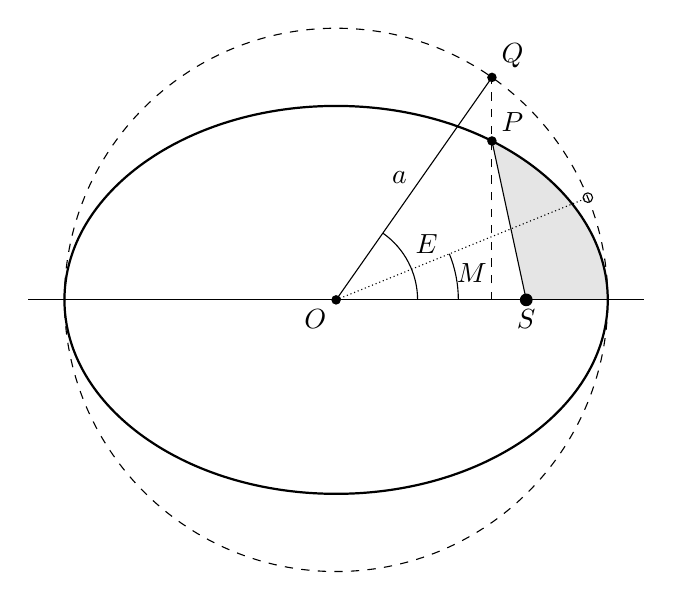
\begin{tikzpicture}[scale=1.15]
% a = 3, epsilon = 0.7, b = 2.142, exzentrische Anomalie E = 55 Grad,
% mittlere Anomalie M = E - epsilon sin E = 22.1 Grad
% ueberstrichene Flaeche
\fill[gray!20] (2.1,0) -- (3,0) arc[start angle=0,end angle=55,x radius=3,y radius=2.142] -- cycle;
% Hilfskreis und Ellipse
\draw[dashed] (0,0) circle (3);
\draw[thick] (0,0) ellipse (3 and 2.142);
\draw (-3.4,0) -- (3.4,0);
% Projektion und Fahrstrahlen
\draw[dashed] (1.721,0) -- (1.721,2.457);
\draw (0,0) -- (1.721,2.457);
\draw (2.1,0) -- (1.721,1.755);
% gleichfoermig laufender Hilfspunkt und Winkel M
\draw[densely dotted] (0,0) -- (2.780,1.129);
\draw (1.35,0) arc[start angle=0,end angle=22.1,radius=1.35];
\node at (1.5,0.3) {$M$};
% Winkel E
\draw (0.9,0) arc[start angle=0,end angle=55,radius=0.9];
\node at (1.0,0.62) {$E$};
% Punkte
\fill (0,0) circle (1.5pt);
\node at (0,0) [below left] {$O$};
\fill (2.1,0) circle (2pt);
\node at (2.1,0) [below] {$S$};
\fill (1.721,1.755) circle (1.5pt);
\node at (1.721,1.755) [above right] {$P$};
\fill (1.721,2.457) circle (1.5pt);
\node at (1.721,2.457) [above right] {$Q$};
\draw (2.780,1.129) circle (1.5pt);
\node at (0.7,1.35) {$a$};
\end{tikzpicture}
\caption{Die Kepler-Gleichung.
Der Planet $P$ läuft auf der Ellipse, die Sonne $S$ steht in einem Brennpunkt, $Q$ ist die Projektion von $P$ auf den Hilfskreis mit Radius $a$, und $E$ ist die exzentrische Anomalie.
Die graue Fläche hat der Fahrstrahl $SP$ seit dem Durchgang durch den sonnennächsten Punkt überstrichen, nach dem Flächensatz ist sie proportional zur Zeit.
Der offene Punkt läuft gleichförmig auf dem Hilfskreis um, sein Winkel ist die mittlere Anomalie $M$, und er bleibt hinter $Q$ zurück, solange sich der Planet von der Sonne entfernt.
\label{bessel:kepler:fig:anomalien}}
\end{figure}
\begin{figure}
\centering
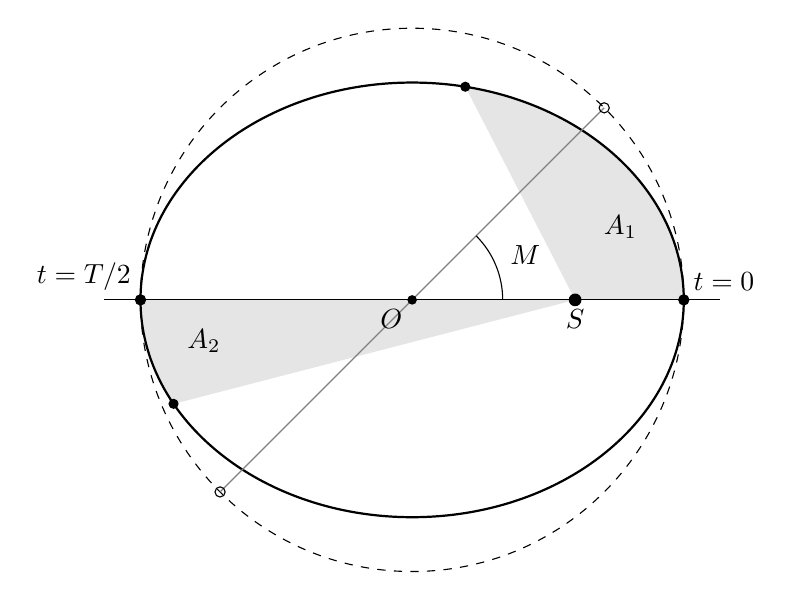
\begin{tikzpicture}[scale=1.15]
% a = 3, epsilon = 0.6, b = 2.4
% zwei Zeitintervalle der Laenge T/8, eines beim Perihel, eines beim Aphel
\fill[gray!20] (1.8,0) -- (3.000,0.000) arc[start angle=0.0,end angle=78.7,x radius=3,y radius=2.4] -- cycle;
\fill[gray!20] (1.8,0) -- (-3.000,0.000) arc[start angle=180.0,end angle=208.6,x radius=3,y radius=2.4] -- cycle;
\node at (2.3,0.8) {$A_1$};
\node at (-2.3,-0.45) {$A_2$};
% Hilfskreis, Ellipse und grosse Achse
\draw[dashed] (0,0) circle (3);
\draw[thick] (0,0) ellipse (3 and 2.4);
\draw (-3.4,0) -- (3.4,0);
% Radien zu den Hilfspunkten, jeweils 45 Grad weiter
\draw[gray] (0,0) -- (2.121,2.121);
\draw[gray] (0,0) -- (-2.121,-2.121);
% Winkel M fuer die Position bei t = T/8
\draw (1.0,0) arc[start angle=0,end angle=45,radius=1.0];
\node at (1.25,0.5) {$M$};
% Positionen des Planeten (gefuellt) und Hilfspunkte (offen)
\fill (3.000,0.000) circle (1.6pt);
\draw (3.000,0.000) circle (1.6pt);
\fill (0.587,2.354) circle (1.6pt);
\draw (2.121,2.121) circle (1.6pt);
\fill (-3.000,0.000) circle (1.6pt);
\draw (-3.000,0.000) circle (1.6pt);
\fill (-2.635,-1.148) circle (1.6pt);
\draw (-2.121,-2.121) circle (1.6pt);
% Sonne und Mittelpunkt
\fill (1.8,0) circle (2pt);
\node at (1.8,0) [below] {$S$};
\fill (0,0) circle (1.5pt);
\node at (0,0) [below left] {$O$};
\node at (3,0) [above right] {$t=0$};
\node at (-3,0) [above left] {$t=T/2$};
\end{tikzpicture}
\caption{Die mittlere Anomalie in zwei gleich langen Zeitintervallen.
Die schwarzen Punkte zeigen den Planeten zu den Zeiten $0$ und $T/8$ sowie $T/2$ und $5T/8$.
Nach dem Flächensatz sind die grau unterlegten Flächen $A_1$ und $A_2$ gleich gross.
Bei $A_1$ legt der Planet dabei einen viel längeren Bogen zurück als bei $A_2$.
Die offenen Punkte auf dem Hilfskreis rücken in beiden Intervallen um denselben Winkel von $45$ Grad vor.
Dieser Winkel ist die mittlere Anomalie $M$, die gleichförmig mit der Zeit wächst.
\label{bessel:kepler:fig:mittlere}}
\end{figure}
Abbildung~\ref{bessel:kepler:fig:mittlere} zeigt beide Bewegungen über einen ganzen Umlauf, der Planet ist in Sonnennähe schnell und in Sonnenferne langsam, der Hilfspunkt läuft gleichförmig.
Der Flächensatz verknüpft die beiden Winkel.
Die Ellipse entsteht aus dem Hilfskreis durch Stauchung um den Faktor $b/a$ senkrecht zur grossen Achse, die graue Fläche in Abbildung~\ref{bessel:kepler:fig:anomalien} ist also das $b/a$-fache der entsprechenden Fläche im Kreis.
Diese besteht aus dem Kreissektor mit Öffnungswinkel $E$ und Flächeninhalt $a^2E/2$ abzüglich des Dreiecks $OSQ$, das die Grundseite $\overline{OS}=a\varepsilon$ und die Höhe $a\sin E$ hat, also den Flächeninhalt $a^2\varepsilon\sin E/2$.
Die graue Fläche ist somit $ab(E-\varepsilon\sin E)/2$, und sie verhält sich zur ganzen Ellipsenfläche $\pi ab$ wie die Zeit $t$ zur Umlaufzeit $T$.
Die kleine Halbachse $b$ kürzt sich dabei heraus, in die Kepler-Gleichung geht nur die Exzentrizität ein.
Das ergibt die \emph{Kepler-Gleichung}
\index{Kepler-Gleichung}%
\begin{equation}
E - \varepsilon\sin E
=
M.
\label{bessel:kepler:eqn:kepler}
\end{equation}
Nach $E$ lässt sie sich nicht auflösen, denn $E$ steht einmal allein und einmal im Sinus, und keine Umformung bringt beides auf eine Seite.
Gesucht ist aber genau das, nämlich $E$ als Funktion der Zeit, denn aus $E$ folgt die Position des Planeten sofort.

Hier kommen die Bessel-Funktionen ins Spiel, und zwar über die Integraldarstellung~\eqref{bessel:eigenschaften:eqn:integral}.
Die Differenz $E-M=\varepsilon\sin E$ ist eine ungerade und $2\pi$-periodische Funktion von $M$, sie lässt sich also in eine Sinusreihe
\begin{equation}
E - M
=
\sum_{n=1}^\infty
b_n\sin nM
\label{bessel:kepler:eqn:sinusreihe}
\end{equation}
entwickeln.
Abbildung~\ref{bessel:kepler:fig:reihe} zeigt diese Funktion für drei Exzentrizitäten, die bewusst grösser gewählt sind als bei den Planeten, weil bei deren kleinen Werten die Kurven vom reinen Sinus nicht zu unterscheiden wären.
Für kleine $\varepsilon$ ist sie fast ein reiner Sinus, mit wachsendem $\varepsilon$ wird sie zunehmend schief, weil der Planet in Sonnennähe schnell läuft und $E$ dort der mittleren Anomalie $M$ davoneilt.
Für die Koeffizienten integriert man partiell und substituiert anschliessend $M=E-\varepsilon\sin E$,
\begin{align}
b_n
&=
\frac{2}{\pi}
\int_0^\pi
(E-M)\sin nM\,dM
\notag
\\
&=
\frac{2}{n\pi}
\int_0^\pi
\biggl(\frac{dE}{dM}-1\biggr)\cos nM\,dM
\label{bessel:kepler:eqn:koeffizienten}
\\
&=
\frac{2}{n\pi}
\int_0^\pi
\cos(nE-n\varepsilon\sin E)\,dE
\notag
\\
&=
\frac{2}{n}\,J_n(n\varepsilon).
\notag
\end{align}
Die Randterme der partiellen Integration verschwinden in~\eqref{bessel:kepler:eqn:koeffizienten}, weil $E-M$ bei $M=0$ und bei $M=\pi$ null ist, und das Integral über $\cos nM$ allein verschwindet ebenfalls.
Im dritten Schritt steht genau das Integral aus~\eqref{bessel:eigenschaften:eqn:integral} mit $x=n\varepsilon$.
Einsetzen in~\eqref{bessel:kepler:eqn:sinusreihe} ergibt die Reihe, die Bessel 1824 gefunden hat \cite{bessel:bessel1824},
\index{Bessel-Reihe}%
\index{Kepler-Gleichung!Bessel-Reihe}%
\begin{equation}
E
=
M
+
2\sum_{n=1}^\infty
\frac{J_n(n\varepsilon)}{n}\,\sin nM.
\label{bessel:kepler:eqn:besselreihe}
\end{equation}

\begin{figure}
\centering
\begin{tikzpicture}
\begin{axis}[
	width=0.95\textwidth,
	height=8cm,
	xmin=0, xmax=6.2832,
	ymin=-0.9, ymax=0.9,
	xtick={0,1.5708,3.1416,4.7124,6.2832},
	xticklabels={$0$,$\pi/2$,$\pi$,$3\pi/2$,$2\pi$},
	ytick={-0.8,-0.4,0.4,0.8},
	axis lines=middle,
	axis line style={-},
	clip=false,
	grid=both,
	grid style={very thin,gray!25},
	legend pos=north east,
	legend cell align=left,
	tick label style={font=\small},
	xticklabel style={yshift=-2pt}
]
\addplot[thick,blue]      table[x=M,y=d02] {papers/bessel/images/kepler.dat};
\addlegendentry{$\varepsilon=0.2$}
\addplot[thick,red]       table[x=M,y=d05] {papers/bessel/images/kepler.dat};
\addlegendentry{$\varepsilon=0.5$}
\addplot[thick,darkgreen] table[x=M,y=d08] {papers/bessel/images/kepler.dat};
\addlegendentry{$\varepsilon=0.8$}
% Bessel-Reihe fuer epsilon=0.8, gestrichelt ein Glied, gepunktet drei Glieder
\addplot[thick,darkgreen,dashed]         table[x=M,y=s1] {papers/bessel/images/kepler.dat};
\addlegendentry{$\varepsilon=0.8$ (1 Glied)}
\addplot[thick,darkgreen,densely dotted] table[x=M,y=s3] {papers/bessel/images/kepler.dat};
\addlegendentry{$\varepsilon=0.8$ (3 Glieder)}
% Achsen über das Gitter hinaus verlängern, wie in den übrigen Abbildungen des Buches
\draw[->] (axis cs:6.2832,0) -- (axis cs:6.65,0) node[below] {$M$};
\draw[->] (axis cs:0,0.9) -- (axis cs:0,1.02) node[right] {$E-M$};
\end{axis}
\end{tikzpicture}
\caption{Die Lösung der Kepler-Gleichung.
Aufgetragen ist die Differenz $E-M=\varepsilon\sin E$ zwischen exzentrischer und mittlerer Anomalie über einen Umlauf, für die Exzentrizitäten $0.2$, $0.5$ und $0.8$.
Sie ist ungerade und $2\pi$-periodisch, und sie wird mit wachsender Exzentrizität immer schiefer, weil der Planet in Sonnennähe schnell und in Sonnenferne langsam läuft.
Gestrichelt und gepunktet ist die Bessel-Reihe~\eqref{bessel:kepler:eqn:besselreihe} für $\varepsilon=0.8$ mit einem und mit drei Gliedern eingezeichnet.
\label{bessel:kepler:fig:reihe}}
\end{figure}

Die Reihe konvergiert für jede Exzentrizität $\varepsilon<1$, also für jede Ellipsenbahn, für $\varepsilon$ nahe bei $1$ allerdings langsam, siehe \cite[Kapitel~XVII]{bessel:watson}.
Das ist bemerkenswert, denn die Entwicklung von $E$ nach Potenzen von $\varepsilon$ konvergiert nur für $\varepsilon<0.6627$, diese Schranke heisst Laplace-Grenze, siehe \cite[S.~270]{bessel:watson} und \cite[Abschnitt~4.8]{bessel:finch}.
\index{Laplace-Grenze}%
Wie langsam die Bessel-Reihe für grosse $\varepsilon$ konvergiert, zeigen die gestrichelte und die gepunktete Kurve in Abbildung~\ref{bessel:kepler:fig:reihe}.
Ein Glied ist ein reiner Sinus und kann die schiefe Form nicht wiedergeben, drei Glieder folgen ihr schon recht gut, und die grösste Abweichung bleibt in Sonnennähe, wo die Kurve am steilsten ist.
Für kleine $\varepsilon$ fallen die Glieder nach~\eqref{bessel:loesung:eqn:kleinx} wie $\varepsilon^n$ ab, und wenige Glieder genügen.
Für die Erde mit $\varepsilon\approx 0.0167$ liefert schon das erste Glied $E\approx M+\varepsilon\sin M$ die exzentrische Anomalie auf rund ein Hundertstel Grad genau.
Damit schliesst sich der Kreis.
Die Integraldarstellung, mit der Bessel seine Funktionen eingeführt hat, ist genau das Werkzeug, mit dem sich die Kepler-Gleichung lösen lässt.
